\section{Spheres}
Let's add a new object: a sphere. The same kind of computations must be applied to a triangle and a sphere. Both are 3D objects, they have a reflectance $\rho$, are made of a specific material (only diffuse for now), have a normal and must be able to compute their intersection with a ray.

Where a triangle is described by its 3 vertices, a sphere has a center C(cx, cy, cz) and a radius R. The intersection between a sphere and a ray is explained below, with P(px, py, pz) the starting point of the ray, $\vec{v}$ the ray direction and I the intersection.

$dx = \vec{v}.x$

$dy = \vec{v}.y$

$dz = \vec{v}.z$

$a = dx^2 + dy^2 + dz^2$

$b = 2 dx (px - cx) + 2 dy (py - cy) + 2 dz (pz - cz)$

$c =  cx^2 + cy^2 + cz^2 + px^2 + py^2 + pz^2 - 2 (cx * pc + cy * py + cz * pz) - R^2$

The discriminant is $d = b^2 - 4 a c$

If $d < 0$ there is no intersection, if $d = 0$ the ray is tangent to the sphere and intersects it in one point, if $d > 0$ the ray intersects the sphere in two points.

To compute the closest intersection, solve our equation by computing m, $m = \frac{-b -\sqrt{d}}{2a}$

This value represents the number of times $\vec{v}$ must be added to P to reach the closest intersection I.

Therefore, I(ix, iy, iz) is

$ix = px + t dx$

$iy = py + t dy$

$iz = pz + t dz$\\


Now that we have our intersections, we must still compute the normal $\vec{n}$ at the intersection to obtain the amount of light reaching our intersection. The normal direction depends on the relative position between the intersection and the center of the sphere. Therefore,

\begin{equation}
\vec{n} = \frac{I - C}{R}
\end{equation}

\begin{figure}[H]
\centering
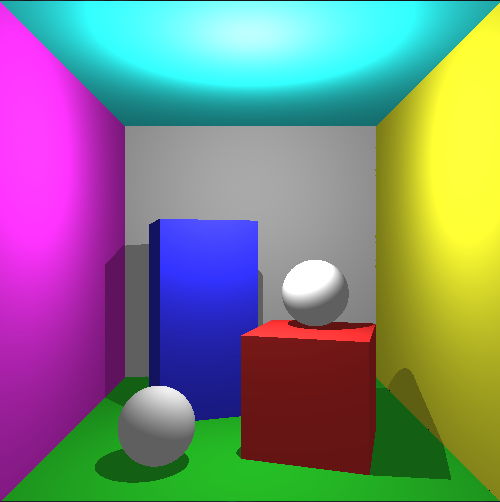
\includegraphics[width=0.35\linewidth]{img/spheres.jpg}
\caption{Spheres (930 ms)}
\end{figure}


\section{Ray-triangle intersection: optimization}
The intersection algorithm is the core of our raytracer and the most called method in our entire program. It is also a bottleneck which could be optimized and lead to great performances.

By trying to reduce the render time of the ray tracer, I found an interesting paper describing a fast ray-triangle intersection algorithm by T. Möller and B. Trumbore \cite{moller2005fast}.

While the algebra used for the calculations is slightly more complex than our previous algorithm, this implementation happens to be way faster, and reduced the render time of the overall process by 2.6 times. Our scene is now rendered in 360 ms instead of 930 ms.


\section{Specular materials}
The performances have been improved but our scene could be better. An interesting effect, which can also be very costly, would be to add specular materials.

The way to do so is quite simple. Previously, the color of a pixel was obtained by multiplying the reflectance of the intersected object to the power light hitting the area, plus the indirect light constant. This procedure won't change, but we now check the material of the intersected object. If it's a specular material, we trace a new ray from the intersection and the color of the pixel will be the one hit by the new ray.

The direction of the new ray is described in equation \ref{eq:specular}, where $\vec{d_i}$ is the incident ray direction, $\vec{n}$ the normal at the intersection and $\vec{d_r}$ the reflected ray direction.

\begin{equation}
\vec{d_r} = \vec{d_i} - 2 (\vec{n} \cdot \vec{d_i}) \vec{n}
\label{eq:specular}
\end{equation}

This operation can be costly if we have many bounces between two specular materials, but it will also give a very nice visual effect. To prevent infinite bounces, we must however limit the maximal number of bounces, and return a default value when this threshold is reached. In the figure below, we can observe the multiple bounces with the left purple wall rendered in the mirror of the tall blue box after a bounce on the specular sphere. The black color reflected is the default color assigned to the "void", i.e. when a ray don't hit any object.

\begin{figure}[H]
\centering
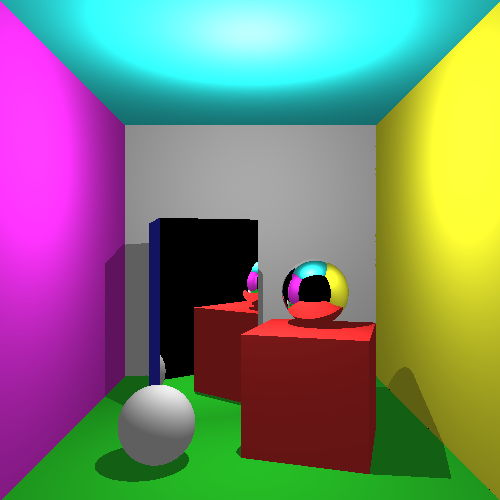
\includegraphics[width=0.35\linewidth]{img/specular.jpg}
\caption{Specular materials}
\end{figure}


\section{Glass - Refraction}
Glass is another interesting material. Yet, this one is tricky since is should refract and reflect rays, each ray having its own percentage of light transmitted according to the incident ray angle. In a first step, we will only implement refraction.

The refraction and reflection formulas to compute those directions and percentages are described in by T Whitted in \cite{whitted1979improved}. However, a faster method, which can actually be proven as equivalent to the previous one using trigonometry and vector algebra, is detailed by PS Heckbert in \cite{heckbert1989derivation}.

The idea lying in those papers is to first compute the cosine angle between the incident vector and the normal at the intersection.

$ cos\theta_1 = \vec{d_i} \cdot \vec{n} $

If the cosine is higher than 0, the incident and normal vectors have the same direction. If so, this means that we are inside the material, so we have already performed a refraction and want to perform a second one. We must therefore use $-\vec{n}$ instead of $\vec{n}$ to compute the next ray direction.

We respectively define $i_1$ and $i_2$ the refractive indices of the current and next material. We remind that $i_{air} \approx 1.0$ and $i_{glass} \approx 1.52$ for most glass materials (nice effects can be obtained by using crystal and caustics, but this feature has not been implemented here).

$\eta = \frac{i_1}{i_2}$

\begin{equation}
cos2\theta_1 = 1 - \eta^2 (1 - cos\theta_1^2)
\label{eq:refraction_percent}
\end{equation}

If $cos2\theta_1$ is lower than 0, the incident ray is completely reflected. This effect, happening when the angle between the incident ray and the normal is higher than a certain threshold, is called \textit{total internal reflection}. $cos2\theta_1$ can actually be approximated as the percentage of light refracted. This is a very useful measure.

The reflected ray direction is then calculated in the same way as in equation \ref{eq:specular}. The refracted ray direction is details in equation \ref{eq:refracted_angle} where $d_R$ is the refracted ray direction.

\begin{equation}
\vec{d_R} = \eta \vec{d_i} + (\eta cos\theta_1 - \sqrt{cos2\theta_1}) \vec{n}
\label{eq:refracted_angle}
\end{equation}

\begin{figure}[H]
\centering
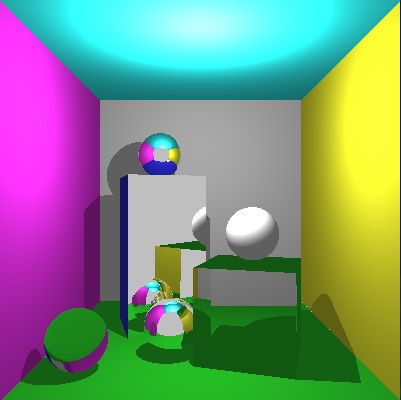
\includegraphics[width=0.35\linewidth]{img/glass_refraction.jpg}
\caption{Refraction through glass (430 ms)}
\label{fig:glass_refraction}
\end{figure}

As specified before, the reflection is not rendered in the previous figure. However, we can observe a total internal reflection with the yellow wall reflected in the mirror after multiple bounces in the glass. Yet, if most of the light should be reflected by the top of the box due to the incident angle, we haven't applied yet the percentage to the refracted ray, which explains the green color.

The smoked glass effect is obtained by reducing the refracted light transmitted by 5\% when entering the object.


\section{Anti-aliasing}
Our scene looks better now. Though the geometry could be improved. Many artifacts could be observed on the edges of figure \ref{fig:glass_refraction}. This aliasing is quite annoying, let's fix it. The following describes various anti-aliasing methods supported by the raytracer. Those algorithms are applied in post-processing, i.e. after the scene has been generated.

\subsection{Edges detection}
Since anti-aliasing can be a costly operation, we want to target only the pixels on the edges, this will avoid an important waste of time.

Instead of displaying a pixel immediately after its computation, we store them in a 2D matrix representing our screen and containing the RGB vector of each pixel. When our scene is complete, we transform this matrix in a grayscale matrix containing values from 0 to 255 instead of RGB vectors. The transformation in equation \ref{eq:grayscale} respects the CCIR 601 recommendations. $I$ is the grayscale intensity, and $\rho$ a RGB vector (reflectance). Figure \ref{fig:grayscale} is the output of this transformation.

\begin{equation}
I = \rho \cdot (0.2989, 0.5870, 0.1140)
\label{eq:grayscale}
\end{equation}

Once we have computed the intensity, we must detect the intensity variations in the scene. This is achieved using the Sobel operator \cite{sobel19683x3}. We define $p_1$ ... $p_9$ the nine values constituting a 3x3 matrix, where $p_1$ is above and to the left, $p_5$ is the pixel itself, and $p_9$ is below and to the right. If the result of equation \ref{eq:sobel} is higher than a threshold (here 0.5), we add the pixel coordinates to a list on which anti-aliasing must be applied. Those pixels are displayed in white in figure \ref{fig:sobel}

\begin{equation}
 g = |( p_1 + 2 * p_2 + p_3 ) - ( p_7 + 2 * p_8 + p_9 )| + |( p_3 + 2 * p_6 + p_9 ) - ( p_1 + 2 * p_4 + p_7 )|
\label{eq:sobel}
\end{equation}

\begin{figure}[H]
\centering
\minipage[t]{0.35\textwidth}
    \centering
    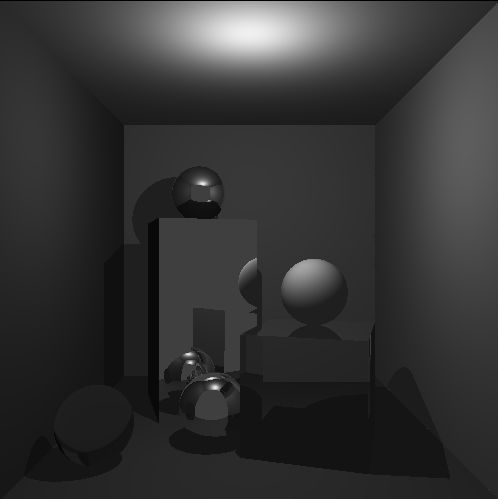
\includegraphics[width=\linewidth]{img/antialiasing/grayscale.jpg}
    \caption{Grayscale scene}
    \label{fig:grayscale}
\endminipage
\minipage[t]{0.35\textwidth}
    \centering
    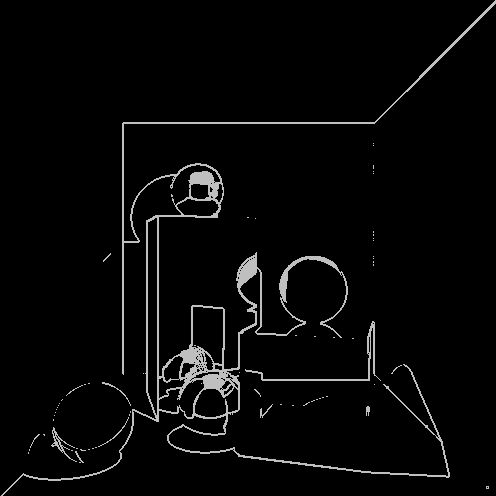
\includegraphics[width=\linewidth]{img/antialiasing/sobel.jpg}
    \caption{Edges detection (Sobel operator)}
    \label{fig:sobel}
\endminipage
\end{figure}


\subsection{Uniform}
Once we know which pixels need anti-aliasing, we can improve the accuracy of our edges by shooting multiple rays in various directions inside each pixel. This process, also called supersampling and illustrated in figure \ref{fig:aa_uniform}, soften the edges by averaging the value of the current pixel and the one of 8 new rays, each ray having the weight $\frac{1}{9}$. Note that the rays must be traced inside the pixel. Averaging the values of the pixels around would only result in a blur instead of improving the accuracy.

\begin{figure}[H]
\centering
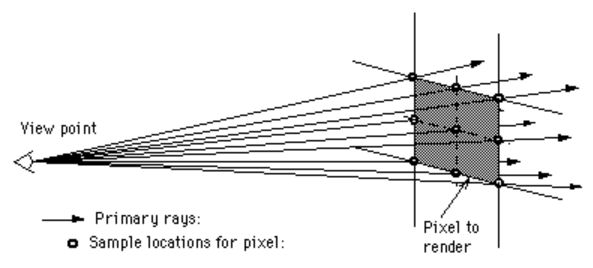
\includegraphics[width=0.5\linewidth]{img/antialiasing/uniform.jpg}
\caption{8 new rays are shot per pixel}
\label{fig:aa_uniform}
\end{figure}

Figure \ref{fig:aa_uniform_zoom} shows the result of this algorithm. The image is a zoom on the mirror after a few forward camera translations and a rotation.

\subsection{Stochastic sampling}
The previous method improves our edges, but the uniform distribution of the rays on the pixel sides preserves the edge geometry and aliasing is still likely to occur.

Since the human eye is very efficient at identifying patterns and their discontinuations, stochastic sampling aims at adding noise to the edges in order to make this task harder, resulting in soften edges perceived. 

To do so, we divide each pixel in a grid, e.g. 4x4 for an anti-aliasing 16x (figure \ref{fig:aa_stochastic}). Instead of only shooting rays on the sides of the pixel, we now shoot one ray per grid cell. The coordinates of the ray shot per cell are randomly sampled inside the cell. We eventually average the value returned by those rays with the current pixel value, each ray having here a weight of $\frac{1}{17}$. Note that we could also ignore the value of the current pixel, but more data is always better.

\begin{figure}[H]
\centering
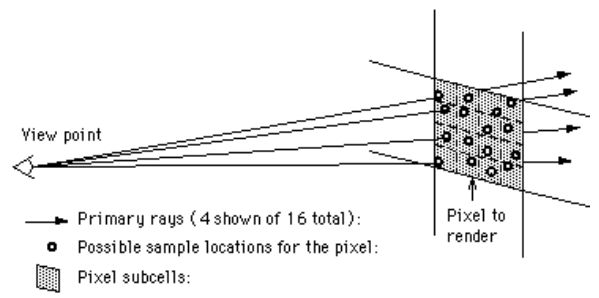
\includegraphics[width=0.5\linewidth]{img/antialiasing/stochastic.jpg}
\caption{16 new rays are sampled on a grid inside each a pixel}
\label{fig:aa_stochastic}
\end{figure}

Our raytracer allows a 2x, 4x, 8x, 16x and 64x anti-aliasing by stochastic sampling.


\subsection{Evaluations}
The following pictures describes the results obtained by some of the previous anti-aliasing algorithms. The computation time is also mentioned.

\begin{figure}[H]
\minipage{0.25\textwidth}
    \centering
    
\includegraphics[width=\linewidth]{img/antialiasing/no_aa.png}
    \caption{AA disabled (430 ms)}
\endminipage\hfill
\minipage{0.25\textwidth}
    \centering
    
\includegraphics[width=\linewidth]{img/antialiasing/super8x.png}
    \caption{Uniform 8x (1200 ms)}
    \label{fig:aa_uniform_zoom}
\endminipage\hfill
\minipage{0.25\textwidth}
    \centering
    
\includegraphics[width=\linewidth]{img/antialiasing/sto8x.png}
    \caption{Jittered 8x (1250 ms)}
\endminipage\hfill
\minipage{0.25\textwidth}
    \centering
    
\includegraphics[width=\linewidth]{img/antialiasing/sto16x.png}
    \caption{Jittered 16x (1450 ms)}
\endminipage\hfill
\end{figure}

\begin{figure}[H]
\centering
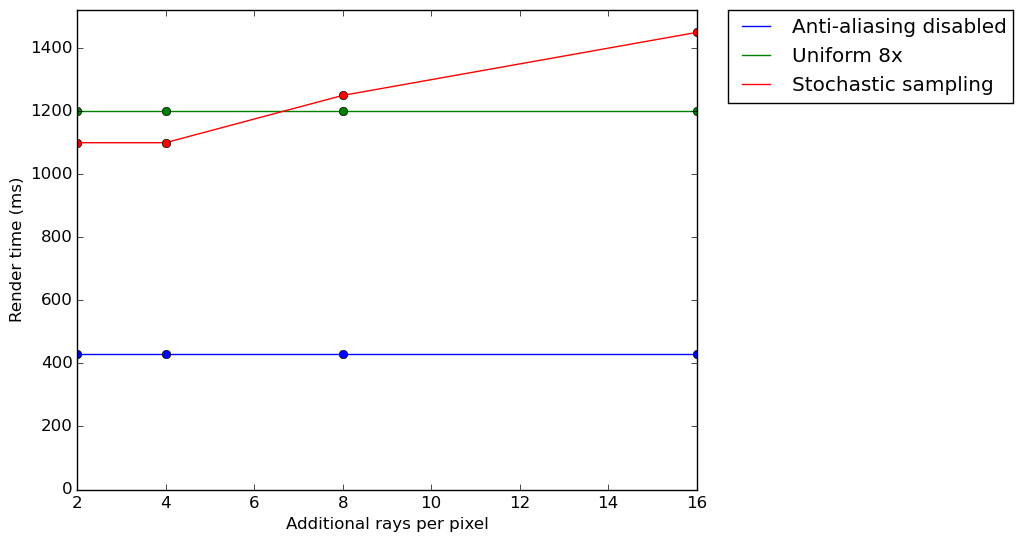
\includegraphics[width=0.4\linewidth]{img/antialiasing/benchmarksAA.jpg}
\caption{Anti-aliasing benchmarks}
\end{figure}


Based on the previous figures and as expected, a stochastic sampling 16x seems to give the best edges.

Another interesting method, not implemented here, is called adaptive sampling. This algorithm shoots 1 ray at each corner of a pixel and then compare their grayscale intensity. If these intensities varies significantly, the pixel is divided into 4 cells and the same algorithm is applied for each cell, until a certain deepness is reached.

\begin{figure}[H]
\centering
\minipage[t]{0.35\textwidth}
    \centering
    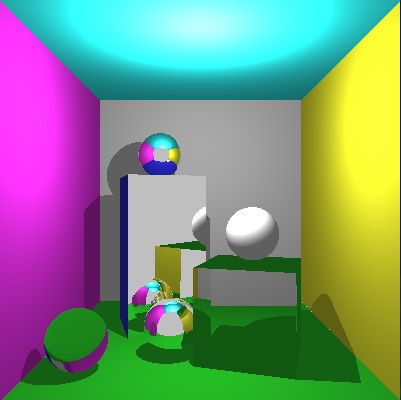
\includegraphics[width=\linewidth]{img/glass_refraction.jpg}
    \caption{Anti-aliasing disabled (430 ms)}
\endminipage
\minipage[t]{0.35\textwidth}
    \centering
    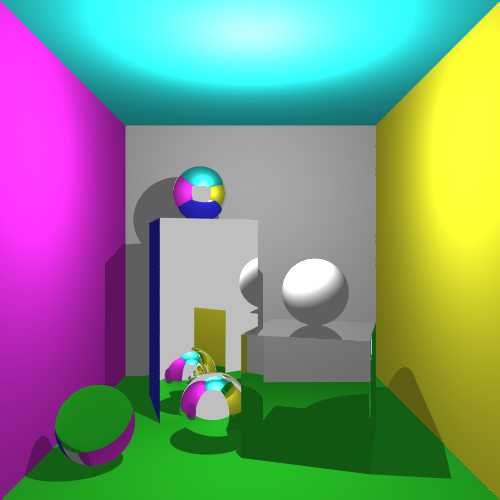
\includegraphics[width=\linewidth]{img/antialiasing/stoAA16x_full.png}
    \caption{Stochastic sampling 16x (1450 ms)}
\endminipage
\end{figure}


\section{Glass - Reflection, diffuse and specular materials}
Our scene is getting good, but we can still add a few improvements. First, we remove the light filter applied on the smoked glass, and replace it with a real percentage (equation \ref{eq:refraction_percent}. We also compute the color of a glass material with equation \ref{eq:glass_full} by shooting a reflected in addition to a refracted ray for each intersection with a glass material. $\rho(I, \vec{v})$ if a function returning the reflectance (RGB color) of a point when shooting a ray from an intersection I in a direction $\vec{v}$. $cos2\theta_1$ is the percentage of refracted light, $\vec{d_R}$ is the refracted vector direction and $\vec{d_r}$ the reflected vector direction.

\begin{equation}
\rho_I = cos2\theta_1 * \rho(I, \vec{d_R}) + (1 - cos2\theta_1) \rho(I, \vec{d_r})
\label{eq:glass_full}
\end{equation}

As for a specular material, we limit the number of bounces. We also change the void color and the color of the diffuse materials.

To make it even better, we introduce a new material, which is diffuse and specular. When a ray will hit this material, a part of the light will be absorbed by the material while some light will bounce like a specular material. The color of such a material is given in equation \ref{eq:diff_spec}, where \textit{r} is the percentage of reflected light, here 0.8. We could also have taken the incident angle into account, but wanted a material more uniform.

\begin{equation}
\rho_I = r \rho_I + (1 - r) \rho(I, \vec{d_r})
\label{eq:diff_spec}
\end{equation}

The result looks great, especially regarding the specular sphere reflected less and less by the glass cube with the number of bounces increasing. This rendering has been computed in 8500 ms with 20 bounces max and anti-aliasing by stochastic sampling 16x. The sphere in the bottom left if made of glass, while the right sphere in the wall is specular.

\begin{figure}[H]
\centering
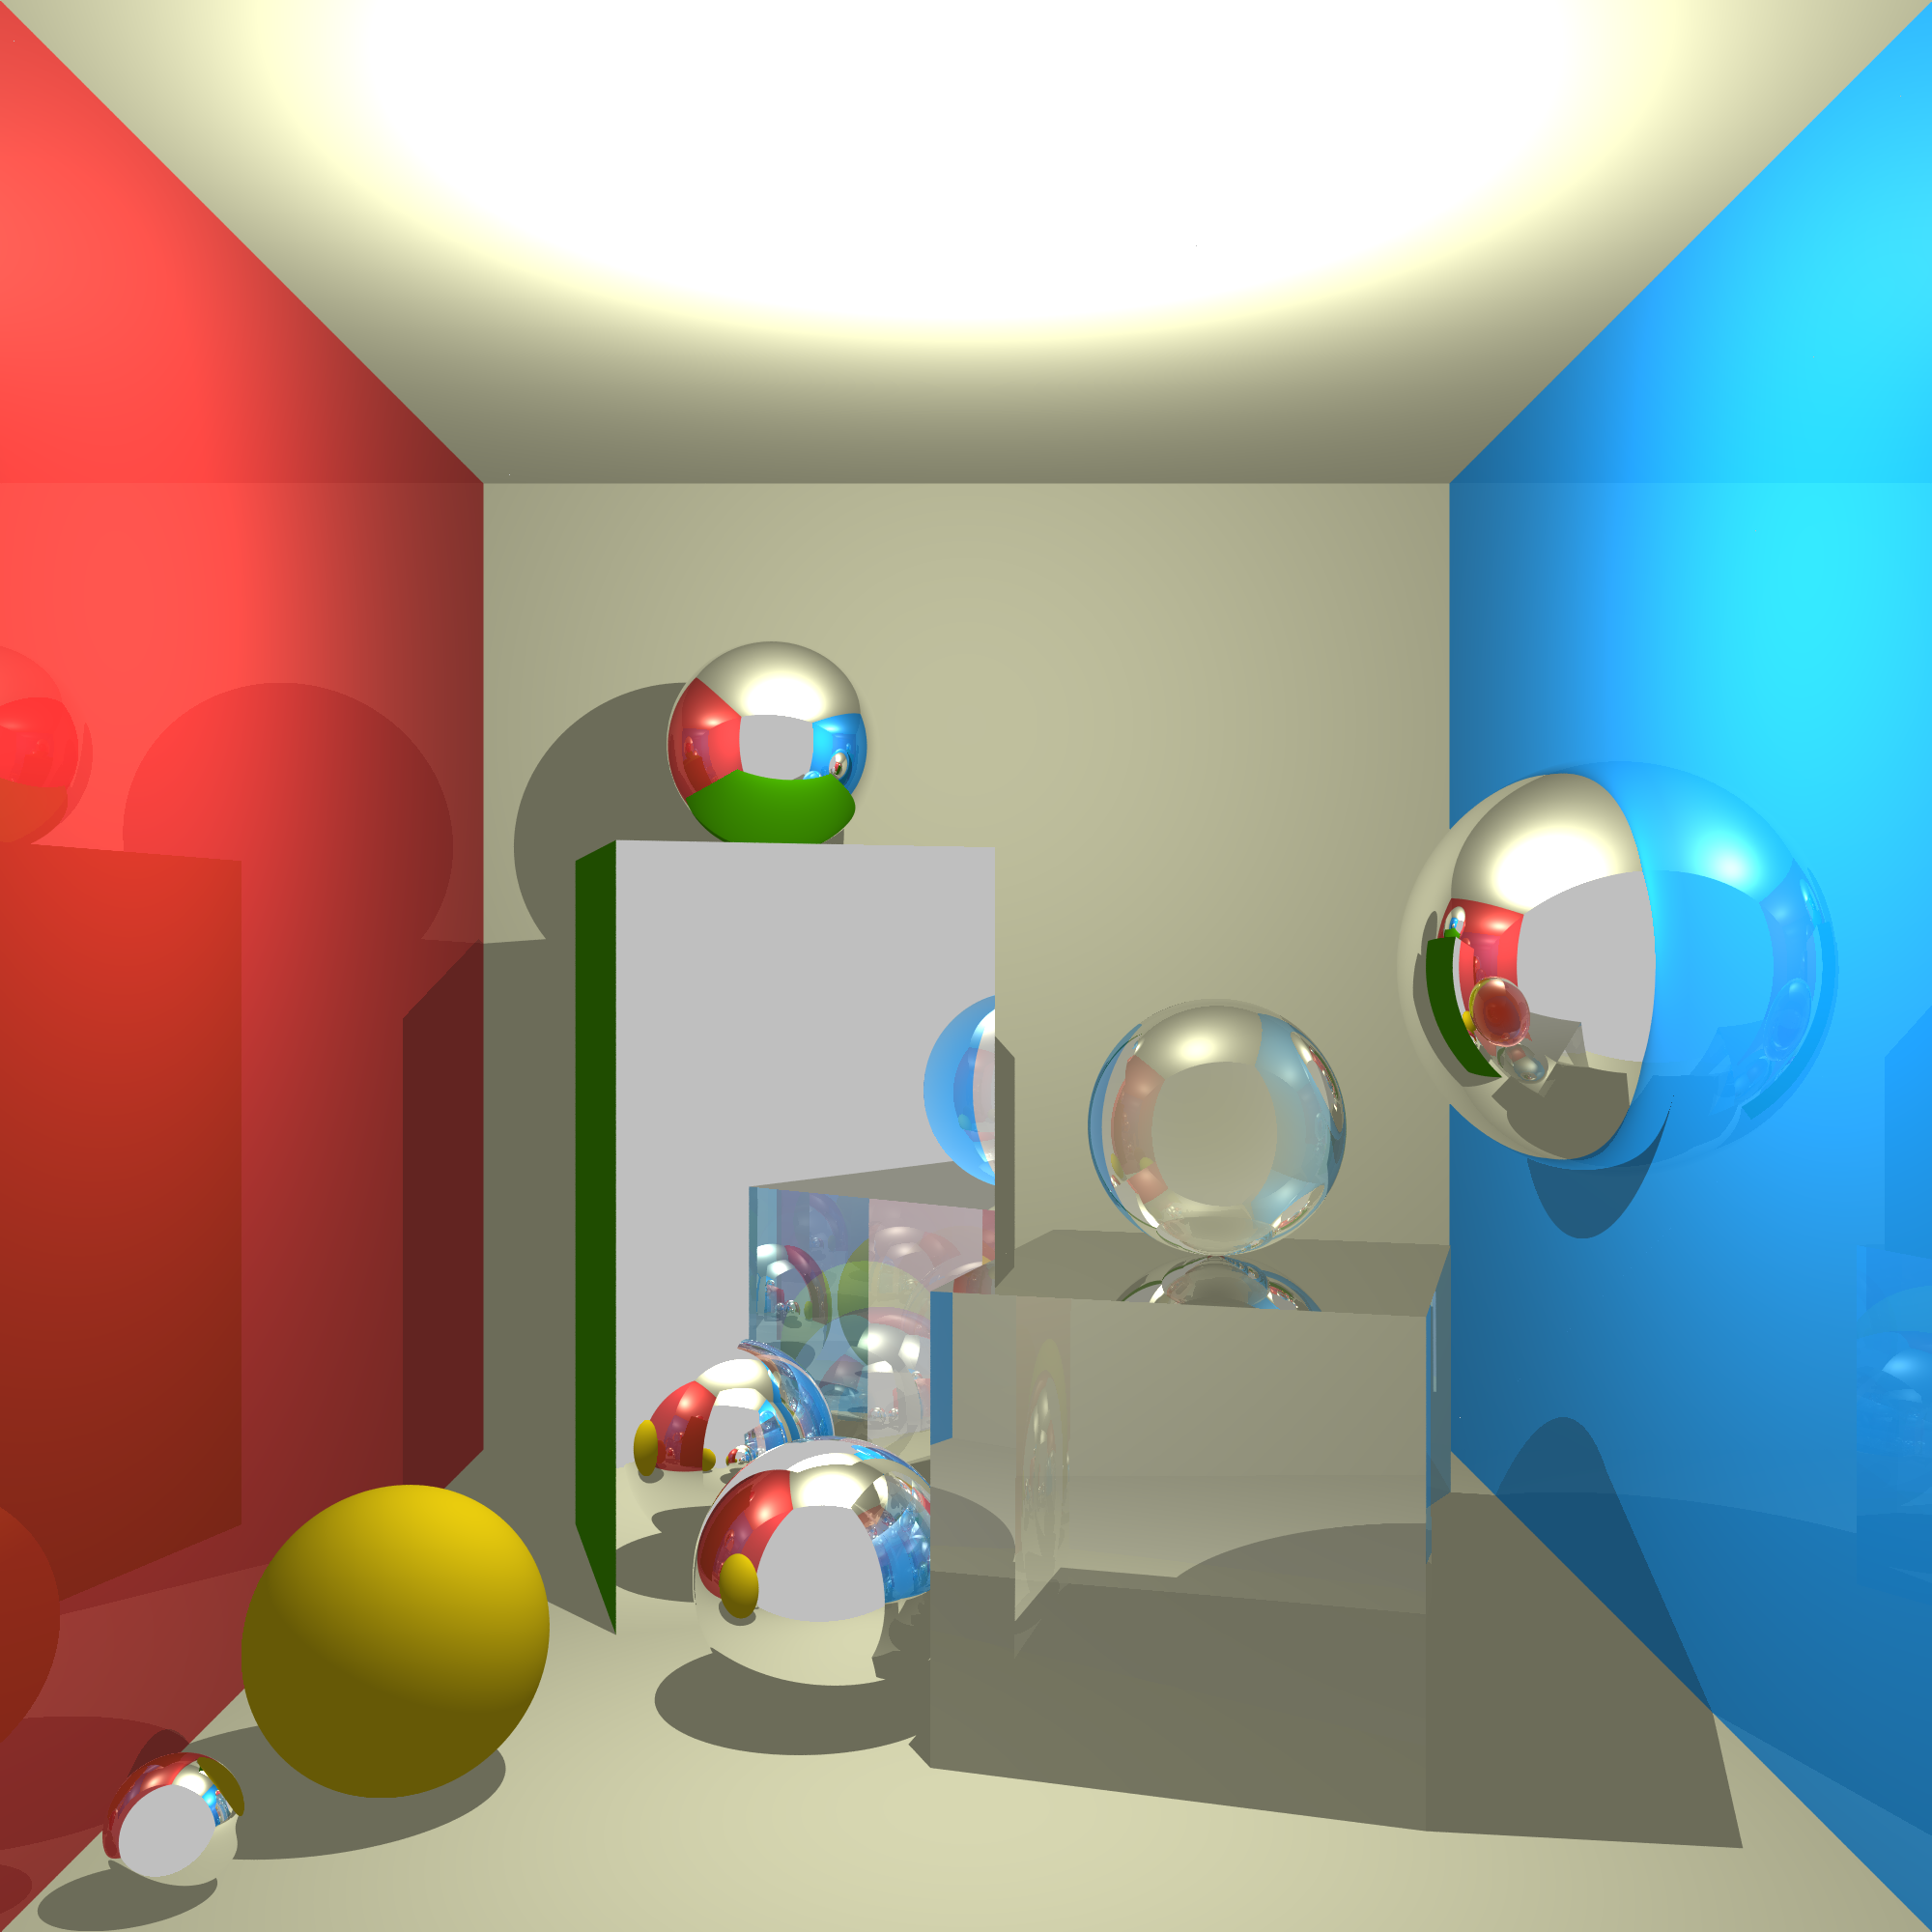
\includegraphics[width=0.35\linewidth]{img/glass_awesome.png}
\caption{Glass: refraction and reflection}
\end{figure}


\section{Soft shadows}
We have a great scene, but the light source looks very unrealistic. Actually, using a single point as light source also results in hard shadows, which could be improved. Let's implement improve it.

We start by adding new triangles to the ceiling of the Cornell Box in order to create a rectangular hole. To prevent that rays going through this whole simply return the void color, we add two other triangles on top of the box. If a ray hit that light surface, we don't compute its illumination according to its color but rather return the light power as a pixel color.

\subsection{Uniform light sources}
Until now, we processed the color of an intersection, multiplied it by the power hitting the intersection (which was (0, 0, 0) if another object was found between the intersection and the light source) and added an indirect illumination vector.

This method won't change, but we now introduce multiple light sources. The previous light position is now considered as the light center. We compute a NxN grid centered on this point, and put a light source in the center of each cell.

\begin{figure}[H]
\centering
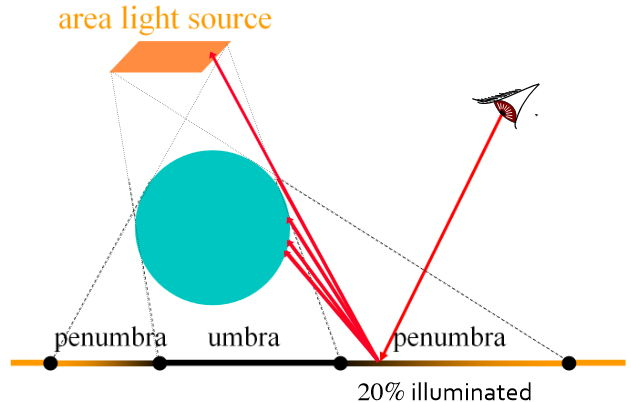
\includegraphics[width=0.4\linewidth]{img/shadows/light1.jpg}
\caption{Soft shadows}
\label{fig:light_uniform}
\end{figure}

In the following equation, $P(I, L_i)$ return the light power hitting an intersection $I$ given a light source $L_i$ according to the light distance and the normal of the object. $(0, 0, 0)$ is returned if the light source cannot be reached. $C$ is the final pixel color.

\begin{equation}
C = \frac{ \sum\limits_{i = 1}^{N*N} P(I, L_i) }{N * N}
\end{equation}

The following scenes were processed in a 500x500 resolution without anti-aliasing.
\begin{figure}[H]
\minipage{0.33\textwidth}
    \centering
    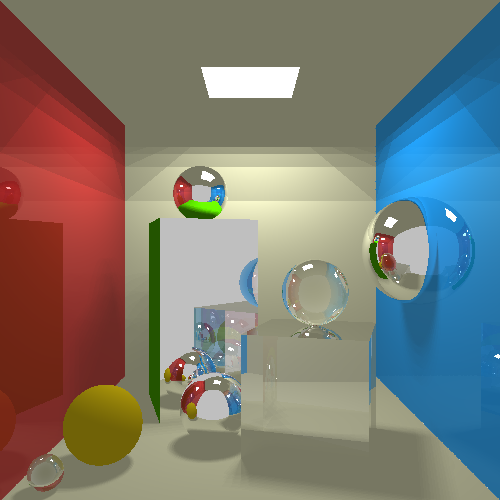
\includegraphics[width=\linewidth]{img/shadows/16.png}
    \caption{16 lights, uniform (8700 ms)}
\endminipage\hfill
\minipage{0.33\textwidth}
    \centering
    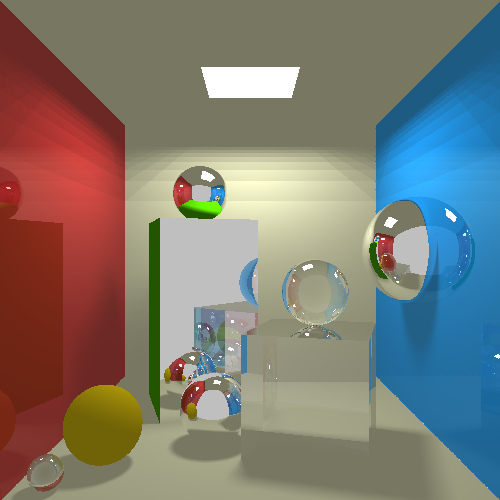
\includegraphics[width=\linewidth]{img/shadows/64.png}
    \caption{64 lights, uniform (30 600 ms)}
\endminipage\hfill
\minipage{0.33\textwidth}
    \centering
    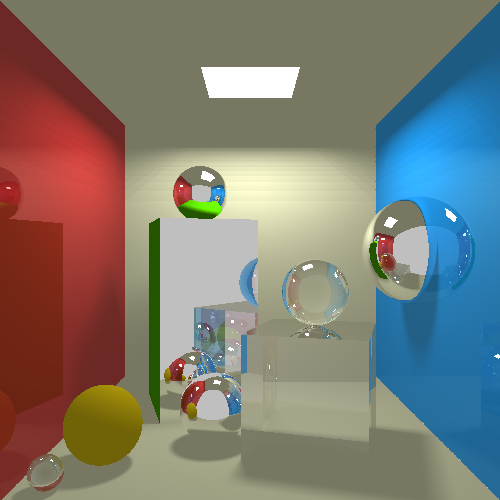
\includegraphics[width=\linewidth]{img/shadows/256.png}
    \caption{256 lights, uniform (118 500 ms)}
\endminipage\hfill
\end{figure}

The computation cost of this technique is high, but the shadows look better. Yet, even with 256 lampes (16x16 grid), we can still see that our light source is composed of multiple light sources.


\subsection{Jittered light sources}
To make it look even smoother we use the same idea as described for the anti-aliasing using stochastic sampling. The grid is of course wider than a pixel, the grid width and height is actually $\frac{1}{6}^th$ of the box size. Instead of having a light in the center of each cell, we now randomly sample the position of each light in the cells.

If done only once, this process would give the same result as before. That's why we sample the light positions for each intersection. This has a small additional cost but the result is way better. Note that if we don't have enough light, shadows are very noisy.

\begin{figure}[H]
\centering
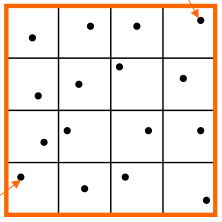
\includegraphics[width=0.25\linewidth]{img/shadows/light2.jpg}
\caption{Light sources jittered by stochastic sampling}
\label{fig:light_jittered}
\end{figure}

\begin{figure}[H]
\minipage{0.33\textwidth}
    \centering
    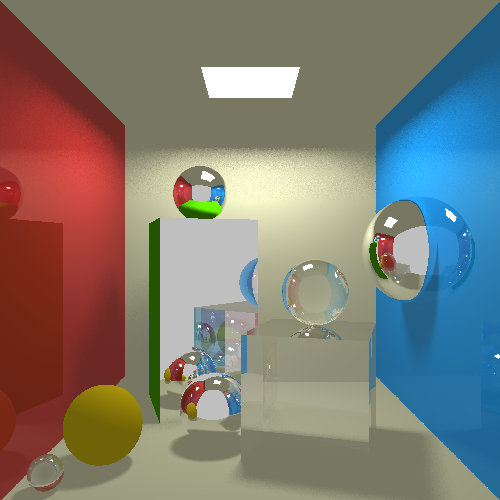
\includegraphics[width=\linewidth]{img/shadows/16_jittered.png}
    \caption{16 lights, jittered (9400 ms)}
\endminipage\hfill
\minipage{0.33\textwidth}
    \centering
    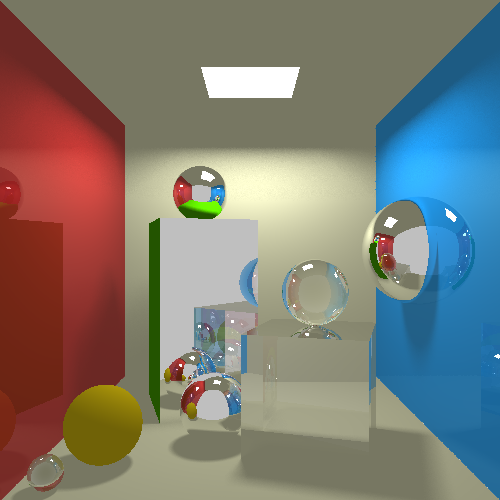
\includegraphics[width=\linewidth]{img/shadows/64_jittered.png}
    \caption{64 lights, jittered (33 600 ms)}
\endminipage\hfill
\minipage{0.33\textwidth}
    \centering
    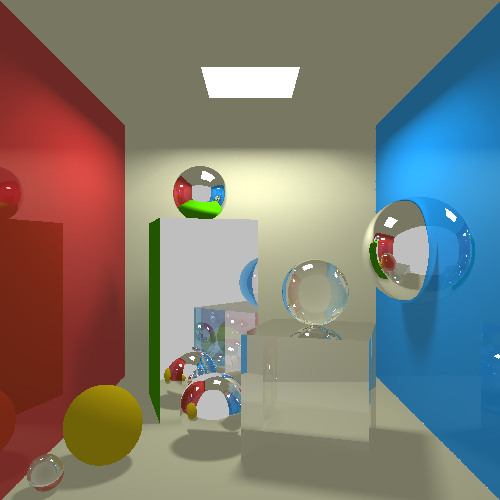
\includegraphics[width=\linewidth]{img/shadows/256_jittered.png}
    \caption{256 lights, jittered (128 600 ms)}
\endminipage\hfill
\end{figure}

Our raytracer support uniform and jittered light sources for any number of lights L distributed on a NxM grid (NxM = L).


\section{Multithreading}
We could stop here, but we want to make our light sources look slightly better. We add a few more rectangles under the hole in the ceiling to make it look like a real light source.

The void is also annoying since it does not support illumination. That's why we extend the walls and close the box behind the camera. We love specular surfaces, so we use the diffuse and specular material for all the walls. Even with limiting the number of bounces, we now have a very very important computation cost, which can take up to a few minutes. Of course, we now stop tracing rays if the percentage of light transmitted is lower that a certain threshold, since that percentage can be very low after bounces in diffuse and specular surfaces. But this is not enough. The solution? Multithreading.

\subsection{Scene processing}
In a first time, we only make parallel the scene processing, i.e. the anti-aliasing stays sequential. Since we iterate through every pixel of our screen in order to trace a ray to get their color, we decide to divide the screens into equal parts, giving each part to a thread. If the number of pixels cannot be divided by the number of threads, we linearly distribute the remaining pixels, i.e. if our screen of 101x101 is divided in a grid of 3x3 threads, the two first threads will in each row and column will have one more pixel in width and height. Each thread has therefore its own width and height, a width and height offset but access to the same pixel matrix as the other threads.

Since each thread writes in its own part of the pixels matrix, two threads will never write in the same pixel, so the screen is not a critical resource. However, a synchronization is needed after processing the scene to sequentially compute the grayscale of the whole pixels matrix.

Multithreading benchmarks are plotted in figure \ref{fig:threading}. Scene is 250x250, 1 uniform light source, 15 bounces max. If an anti-aliasing is used, it's stochastic sampling 16x. Computations are performed on a quad-core hyperthreaded. The \textit{No AA} curve shows a nice speedup when increasing the number of threads. However, by looking at the \textit{Sequential AA} curve, it's quite obvious that we have too much sequential code in our implementation when using anti-aliasing.

\subsection{Anti-aliasing}
We improve our performances by building a list containing the coordinates of the pixels needing anti-aliasing, and dividing this list into equal parts assigned to each thread (we actually don't divide the list, but give an offset and number of pixels to compute to each thread). Each pixel eventually compute anti-aliasing for each thread it has been assigned.

A synchronization is set after computing the anti-aliasing, since displaying pixel on the screen is a sequential code due to the fact that the screen is a critical resource.

\begin{figure}[H]
\centering
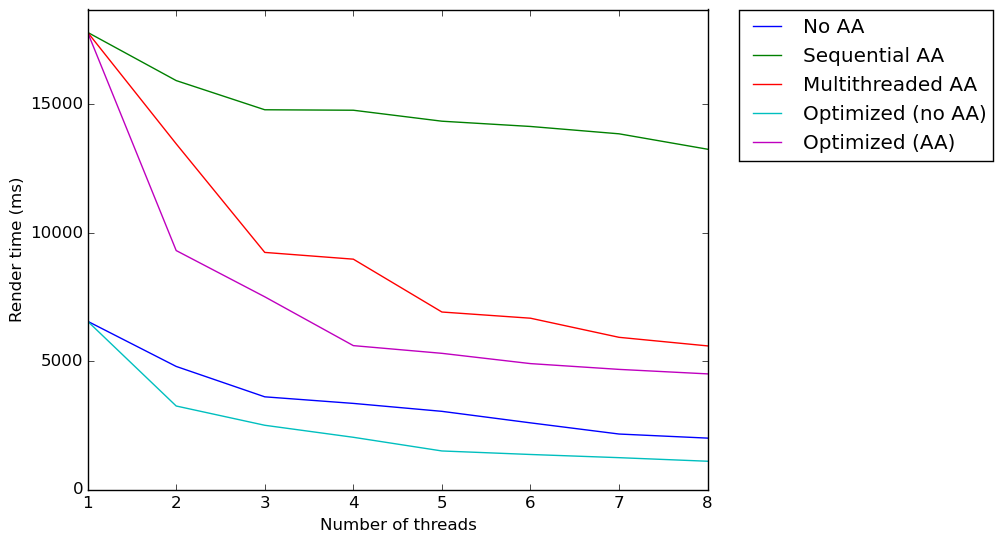
\includegraphics[width=0.4\linewidth]{img/benchmarksThreads.jpg}
\caption{Multithreading benchmarks}
\end{figure}

The \textit{Multithreaded AA} curve looks better than the previous ones. Yet, about 30\% of the time elapsed is wasted by waiting at the synchronization barrier. Indeed, some parts of the scene are longer to compute than others, and the thread responsible for the part containing the two specular surfaces and the glass cube has to compute a lot more bounces.

\subsection{}

\begin{figure}[H]
\centering
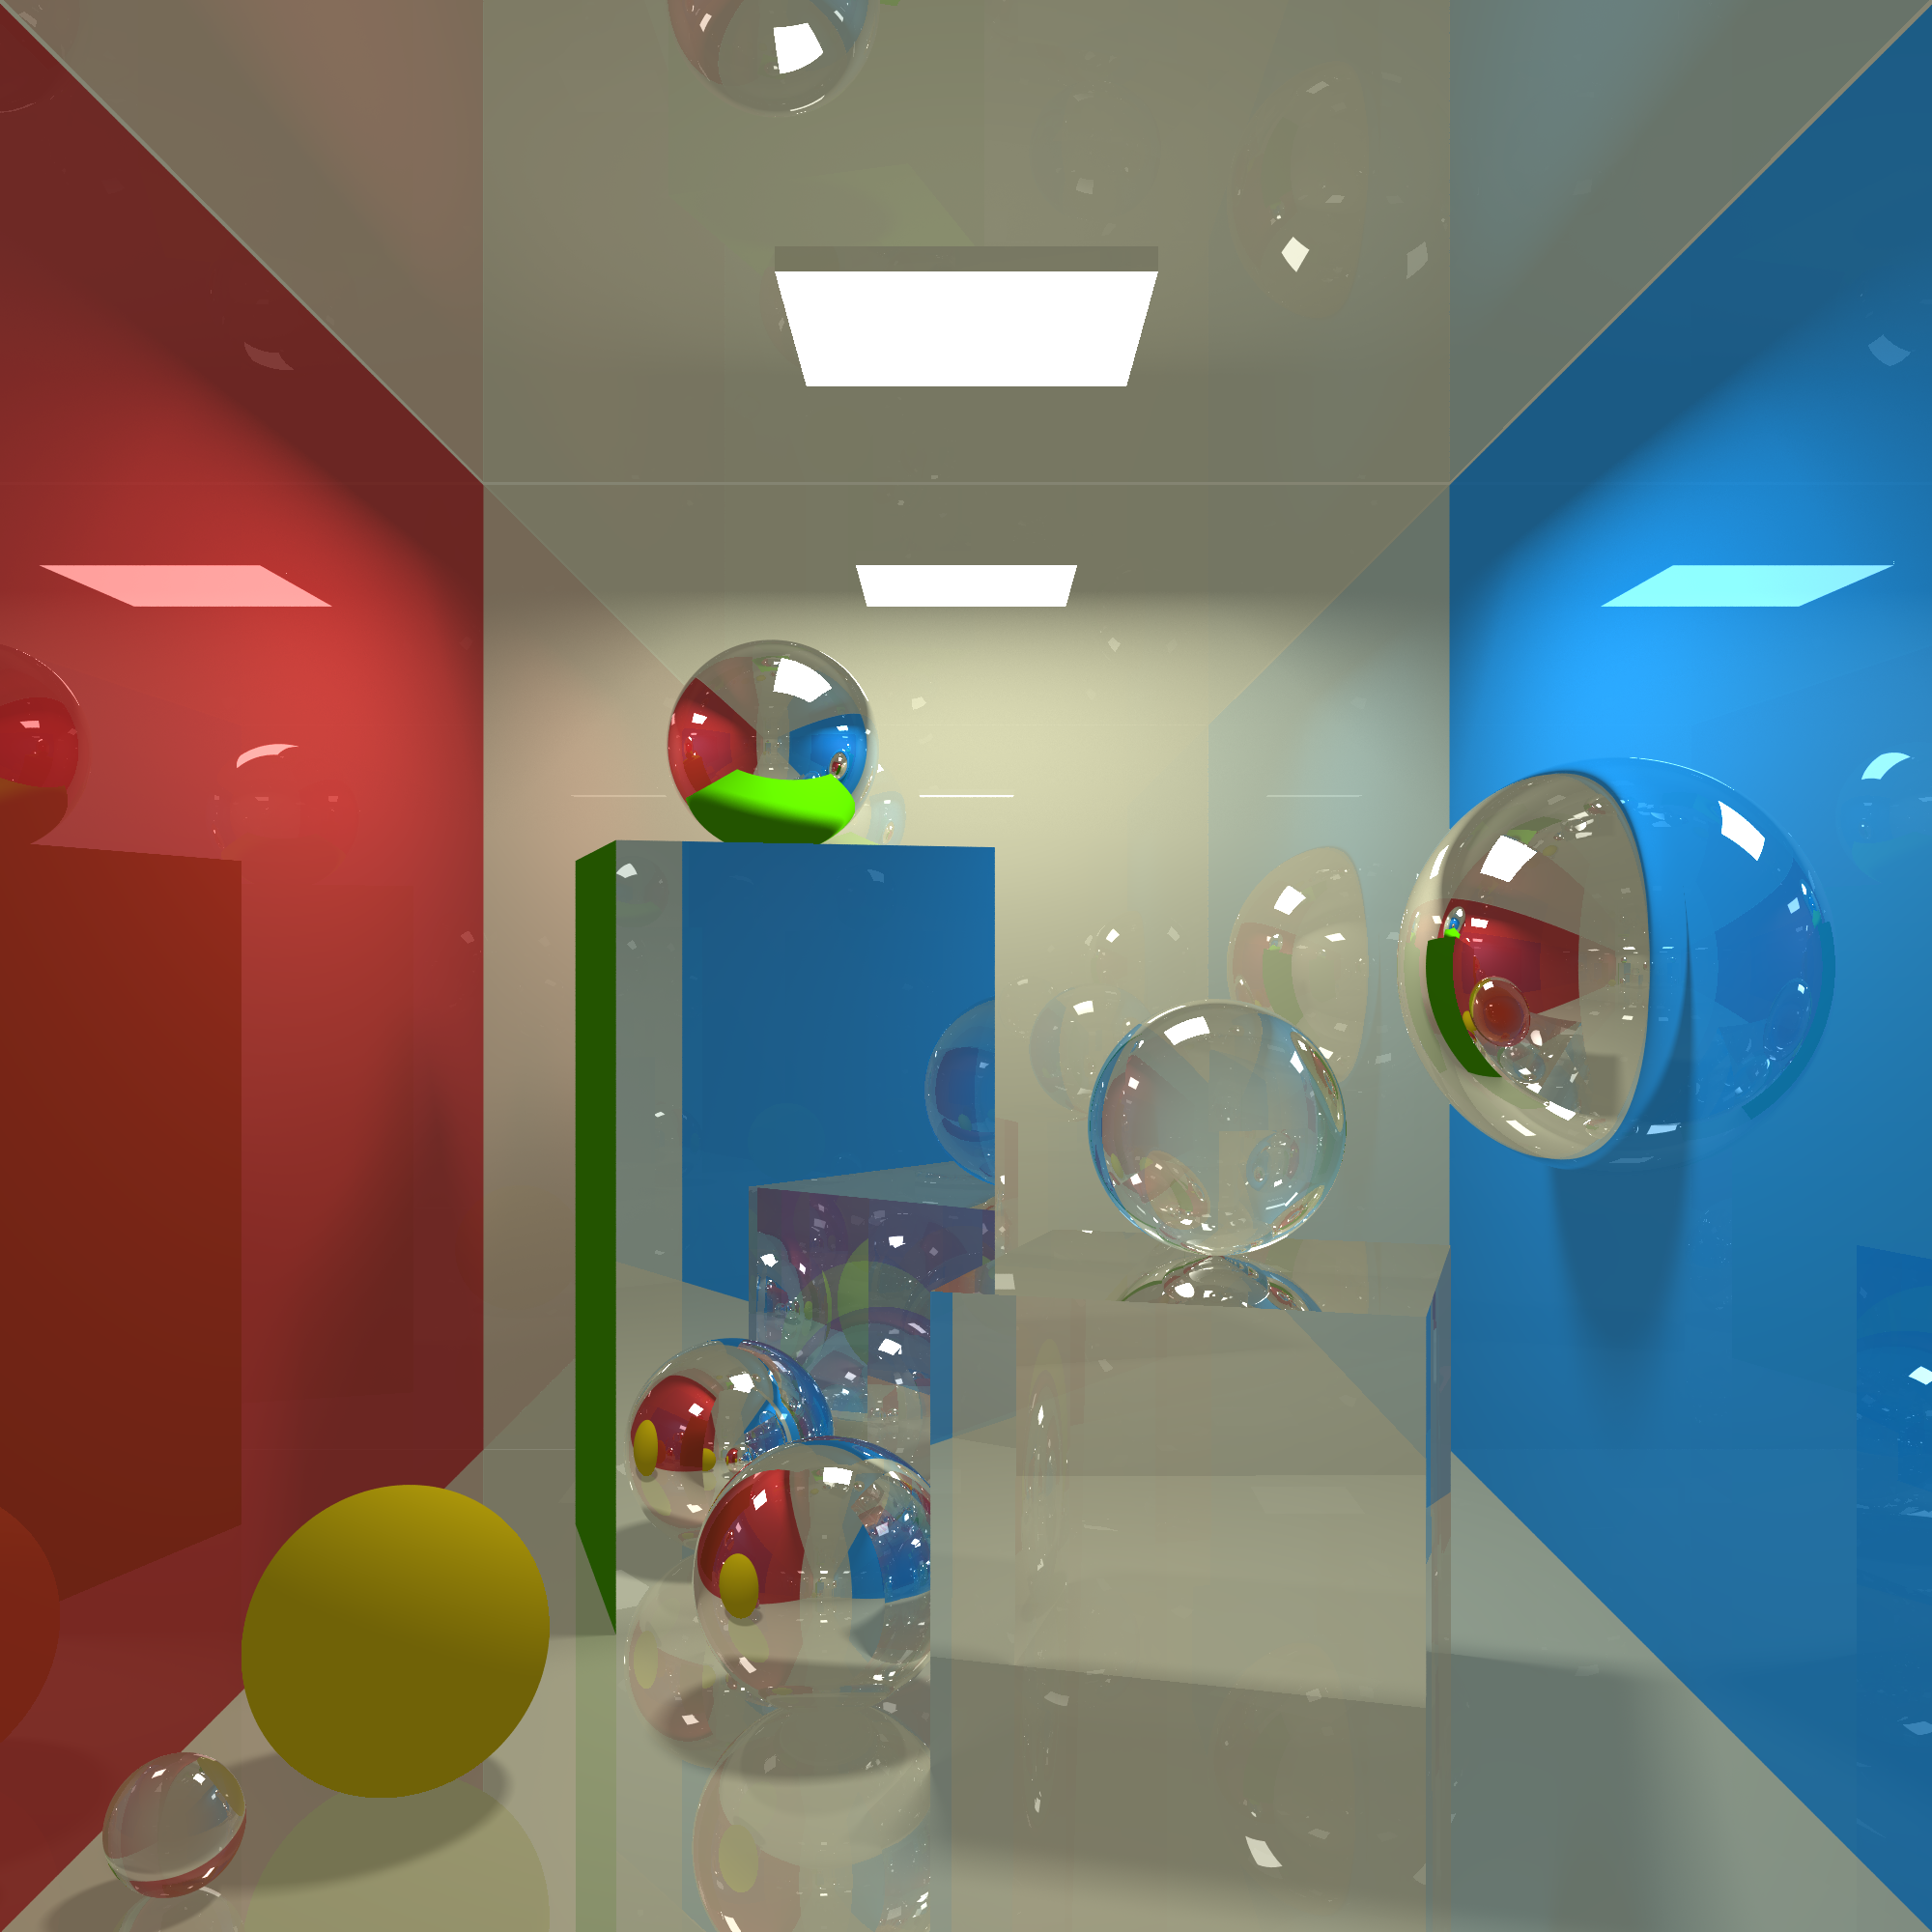
\includegraphics[width=0.6\linewidth]{img/final.png}
\caption{Final scene}
\end{figure}
